\documentclass{beamer}

\usepackage[style=numeric, natbib]{biblatex}
\usepackage{caption}
\usepackage{color}
\usepackage{amsmath}
\usepackage{array}
\usepackage{booktabs}
\usepackage{caption}
\usepackage{fancyvrb}
\usepackage{graphicx}
\usepackage{longtable}
\usepackage{newtxmath}
\usepackage{tabularx}
\usepackage{zi4}
\usepackage{graphicx}
\usepackage{colortbl}
\usepackage{microtype}
\usepackage{balance}
\usepackage{mathtools}
\usepackage{float}
\usepackage{listings,lstlangcoq}
\usepackage{xcolor}
\usepackage{centernot}
\usepackage{soul}
\usepackage[all]{xy}

\lstset{language=sh,
  basicstyle=\footnotesize\ttfamily,
  keywordstyle=\footnotesize\color{blue}\ttfamily,
  moredelim=**[is][\btHL]{|}{|},
  escapeinside={<@}{@>}
}

\usetheme{Antibes}
\usecolortheme{beaver}

\addbibresource{references.bib}

\title{CFG Patterns: A new tool to formally verify optimizations in Vellvm}

\author[Léon Frenot]{Leon Frenot\\ Supervised by Yannick Zakowski \& Gabriel Radanne}

\date[July 12th, 2024]{February 5th, 2024 - July 5th, 2024}

% \setbeamertemplate{footline}[frame number]
\setbeamertemplate{navigation symbols}{}

\makeatletter
\setbeamertemplate{footline}{
  \leavevmode%
  \hbox{%
    \begin{beamercolorbox}[wd=.333333\paperwidth,ht=2.25ex,dp=1ex,center]{author in head/foot}%
      \usebeamerfont{author in head/foot}\insertshortauthor
    \end{beamercolorbox}%
    \begin{beamercolorbox}[wd=.333333\paperwidth,ht=2.25ex,dp=1ex,center]{title in head/foot}%
      \usebeamerfont{title in head/foot}\insertshortdate
    \end{beamercolorbox}%
    \begin{beamercolorbox}[wd=.333333\paperwidth,ht=2.25ex,dp=1ex,right]{date in head/foot}%
      \insertframenumber{} / \inserttotalframenumber\hspace*{2ex}
    \end{beamercolorbox}%
  }%
  \vskip0pt%
}
\makeatother

\lstdefinestyle{customcoq}{
  columns=flexible,
  mathescape=true,
  belowcaptionskip=1\baselineskip,
  breaklines=true,
  xleftmargin=\parindent,
  language=Coq,
  morekeywords={Variant, fun, Arguments, Type, cofix},
  % morekeywords={SOCKAPI,ITREE,data_at,data_at_},
  emph={%
      SOCKAPI,ITree,data_at,data_at_
    },
  emphstyle={\bfseries\color{green!40!red!80}},
  showstringspaces=false,
  basicstyle=\small\ttfamily,
  keywordstyle=\bfseries\color{green!20!black},
  commentstyle=\itshape\color{red!40!black},
  identifierstyle=\color{violet!50!black},
  stringstyle=\color{orange},
  escapeinside={<@}{@>}
}
\newcommand{\inlinecoq}[1]{\mbox{\lstinline[style=customcoq,columns=fixed,basewidth=.48em]{#1}}}
\newcommand{\ilc}[1]{\inlinecoq{#1}}

\newcommand{\leon}[1]{\textcolor{blue}{#1}}
\newcommand{\gr}[1]{\textcolor{Orange}{#1}}
\newcommand{\yz}[1]{\textcolor{ForestGreen}{#1}}
\newcommand{\yzt}[1]{\textcolor{ForestGreen!50}{#1}}
\newcommand{\cut}[1]{\textcolor{Gray!40}{#1}}
\newcommand{\ocfg}{OCFG\xspace}
\newcommand{\pat}{\texttt{Pat}\xspace}

\begin{document}

\frame{\titlepage}

% \begin{frame}
%   \begin{block}{Context}
%     \begin{itemize}
%       \item M2 research internship
%       \item 5 Months in LIP Computer Science laboratory at ENS Lyon.
%       \item Compilation and Analysis, Software and Hardware Team.
%     \end{itemize}
%   \end{block}
%   \begin{block}{Keywords}
%     \begin{itemize}
%       \item Verified Compilation
%       \item Verified Code transformations
%       \item DSL of patterns
%     \end{itemize}
%   \end{block}
%   \leon{Enlever}
% \end{frame}

\section{Introduction}

% \begin{frame}{Table of Contents}
%   \tableofcontents
% \end{frame}

\subsection*{Motivation}

\begin{frame}{Motivation}
  Critical sectors: code as bug-free as possible.\\
  Important part of the toolchain: compilation.\\
  Compilers are also very complex objects. gcc: 15 million lines of code.
  \begin{block}{How to remove bugs introduced by compilation?}
    \begin{itemize}
      \item Compile without optimization, and manually go through the generated machine code to ensure it follows the original code,
      \item or use verified compilers.
    \end{itemize}
  \end{block}
\end{frame}

\begin{frame}{Verified compilers}
  Compilers written inside of a proof assistant, for example Coq, and proven correct with the tools it provides.
  \begin{itemize}
    \item CompCert (2009), verified compiler for the ISO C 99 language,
    \item Vellvm (2021), verified compiler project for LLVM IR.
  \end{itemize}
\end{frame}

\subsection*{Background: LLVM}

\begin{frame}{LLVM IR}
  \begin{figure}
    \scalebox{.85}{\xymatrix{
      &Front-end&&Back-end\\
      C\ar[r]&*+[F]{Clang}\ar@(r,l)[dr]&&&x86\\
      Rust\ar[r]&*+[F]{rustc}\ar[r]&LLVM\ IR \ar@(ul,ur)[]^{\txt{optimization\\passes}} \ar[r]&*+[F]\txt{LLVM\\Compiler} \ar@(r,l)[ur]\ar[r]\ar@(r,l)[dr]&ARM\\
      Go\ar[r]&*+[F]{Gollvm}\ar@(r,l)[ur]&&&RISC-V
      \save "1,2"."4,2"*+[F--]\frm{} \restore
      \save "1,4"."4,4"*+[F--]\frm{} \restore
    }}
  \end{figure}
\end{frame}

\begin{frame}{}
  \begin{figure}
    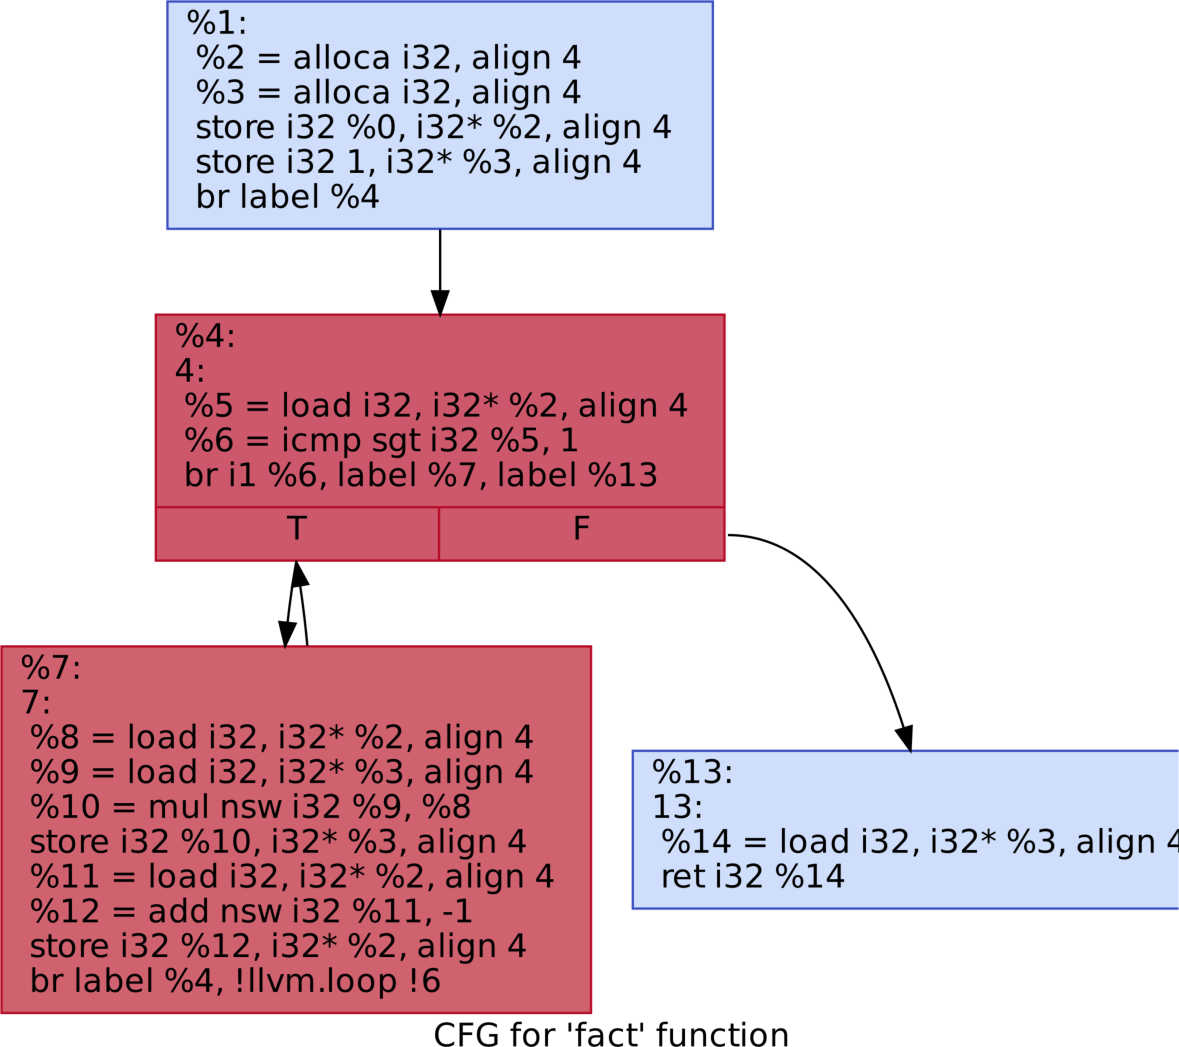
\includegraphics[height=.8\textheight]{images/output2.pdf}
    \caption{An LLVM function}
  \end{figure}
\end{frame}

\begin{frame}{LLVM IR}
  \begin{itemize}
    \item Intermediate representation for multiple frontends and backends.
    \item RISC-like instruction set with high-level informations.
    \item Features:\begin{itemize}
            \item SSA form guarantee
            \item named labels and registers
            \item integer-pointer casts
            \item analysis and transformation passes
          \end{itemize}
    \item Vellvm: formally define LLVM IR's semantics and build verified components.
  \end{itemize}
\end{frame}

\subsection*{Goal of the internship}

\begin{frame}
  \begin{block}{Goal of the internship}
    Formally verify optimizations in Vellvm
  \end{block}

  \begin{itemize}
    \item Identify a subgraph with specific structural properties.
    \item Link the transformed subgraph back with the context.
  \end{itemize}
  % \leon{DSL Pat, matcher, implementation, preserve semantics, generic substitution theorem}
\end{frame}

\begin{frame}{Contributions}
  \begin{itemize}
    \item Designed and implemented a DSL of patterns over graphs, Pat.
    \item Equipped it with a matcher that computes the set of decompositions that match a given pattern in a given graph.
    \item Proved a generic substitution theorem.
    \item Leveraged it and the specifications given by Pat to establish a proof for an optimization.
  \end{itemize}
\end{frame}

\begin{frame}
  \begin{figure}
    \scalebox{.8}{\xymatrix{
      &&&\txt{LLVM IR}\ar[dd]^{\txt{Parsing}}\\
      &&*+[F]{\txt{Coq\\Vellvm}}\\
      *+[F]{\mathcal{T}}&\txt{Analysis}\ar[dd]&&*+[F--]{\txt{OCFG}}\ar@{=>}[r]^{\llbracket\ldots\rrbracket} \ar[dd]^{\mathcal{T}} & *+[F--]{\txt{ITrees\\Semantic}}\ar@{~}@<-2pt>[dd]\ar@{~}@<+2pt>[dd]^{Bisimilarity}\\
      &&&\ar@(l,r)[ull]_{\txt{Pattern}}\ar@(l,r)[dll]^{\txt{Substitution}}\\
      &\txt{Emission}&&*+[F--]{\txt{OCFG}}\ar@{=>}[r]^{\llbracket\ldots\rrbracket} \ar[dd]^{\txt{Printer}} & *+[F--]{\txt{ITrees\\Semantic}}\\
      &&&&&&\\
      &&&\txt{LLVM IR}
      \save "2,3"."6,6"*+[F]\frm{} \restore
      \save "3,1"."5,2"*+[F]\frm{} \restore
    }}
  \end{figure}
\end{frame}

\section{An example of optimization: Block Fusion}

\begin{frame}{Table of Contents}
  \tableofcontents
\end{frame}

\begin{frame}{Block Fusion}
  \begin{figure}
    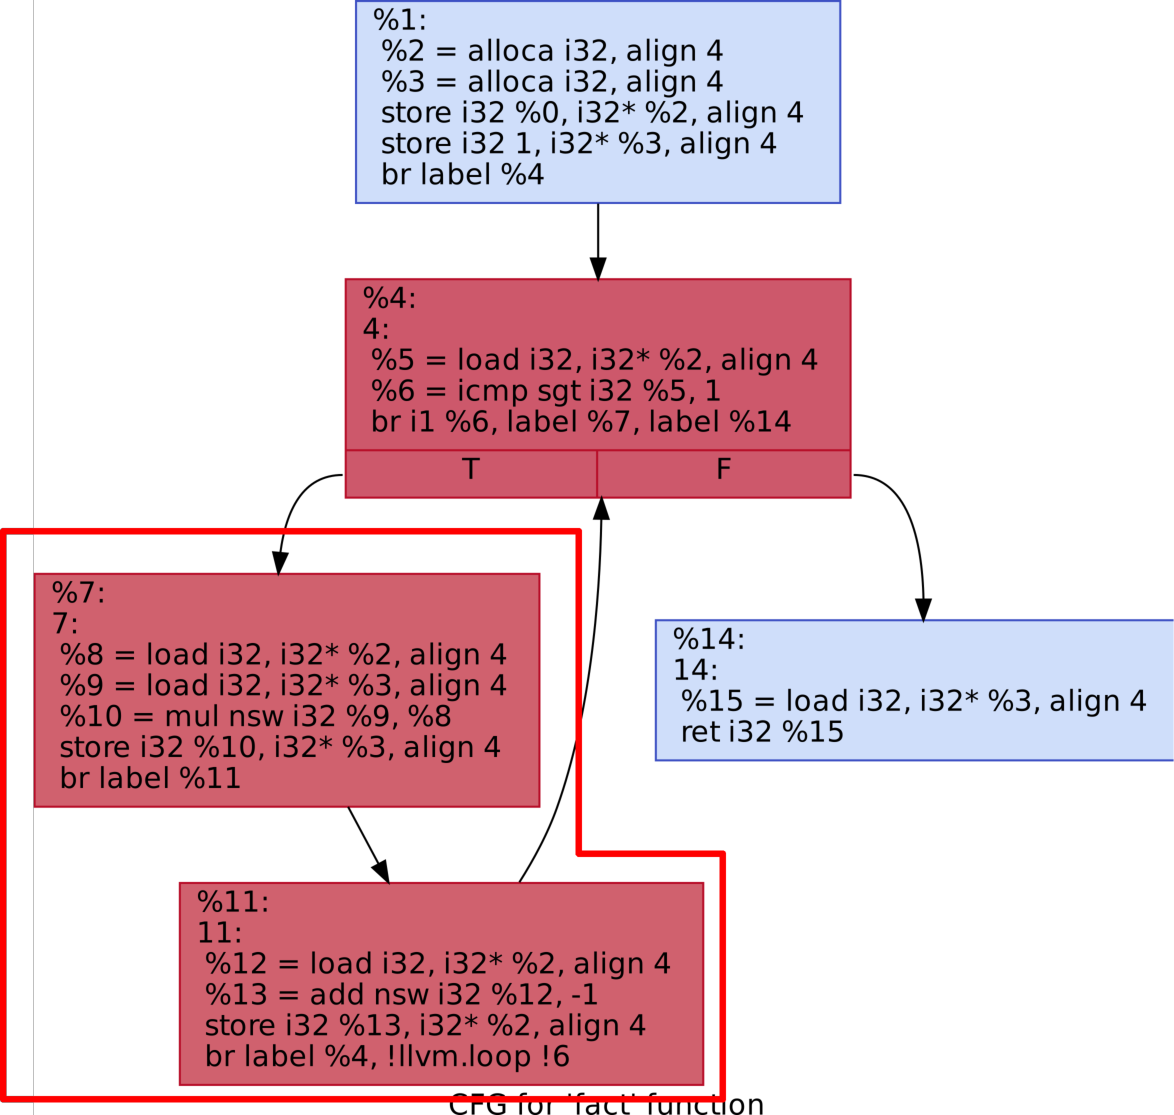
\includegraphics[width=.45\textwidth]{images/output.pdf}
    \centering $\implies$
    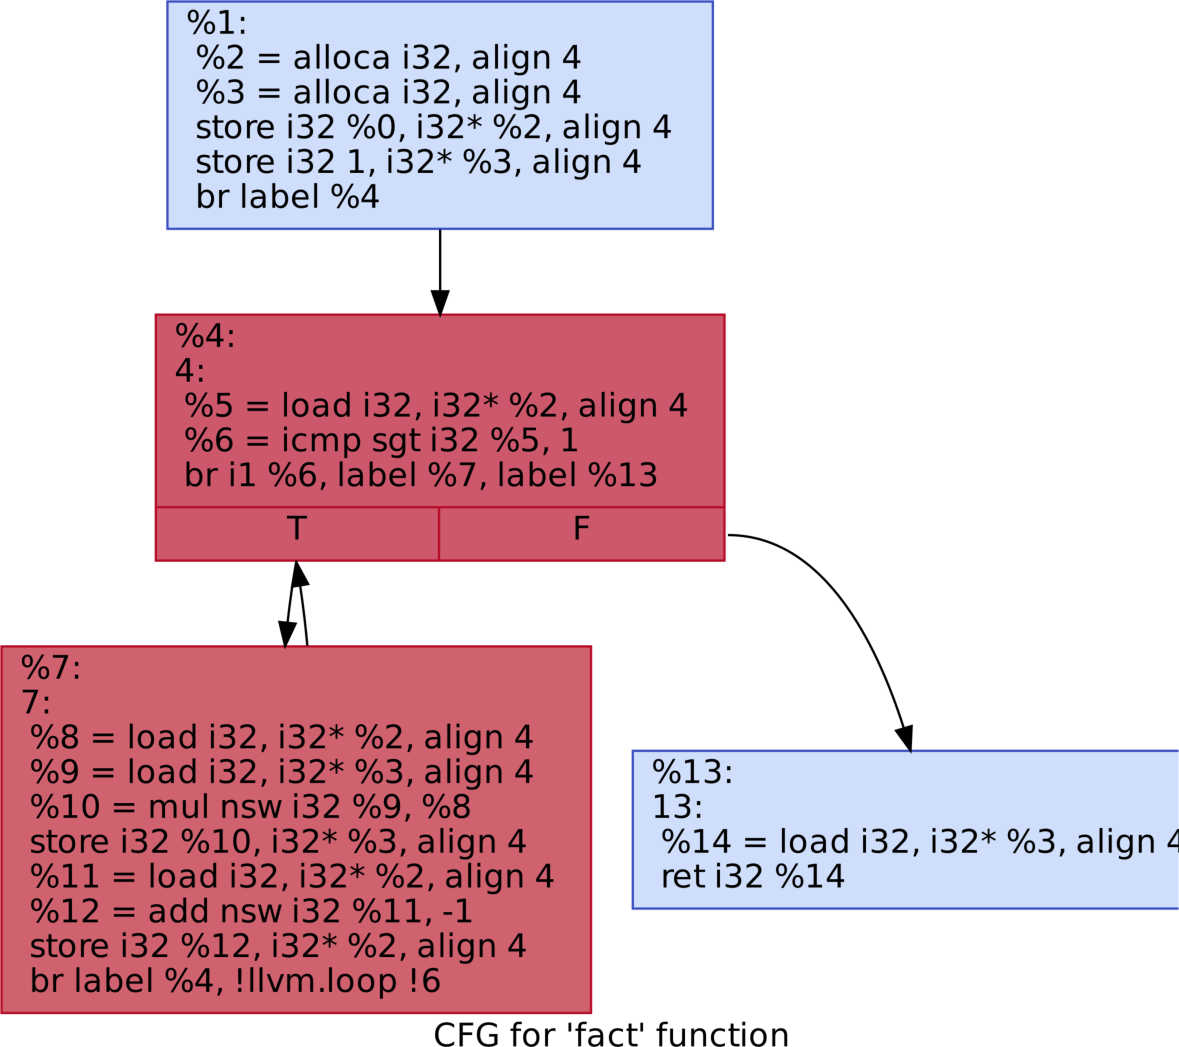
\includegraphics[width=.45\textwidth]{images/output2.pdf}
    \caption{Applying Block Fusion to a CFG}
  \end{figure}
\end{frame}

\begin{frame}[fragile]{A pattern for Block Fusion}
  \begin{figure}
    \scalebox{0.75}{\xymatrix{
    &&&&\\
    &*+[F]\txt{\ilc{A}\\\ilc{Block}: any block}\ar[dd]&&\;\ar@{-->}`u[ul] `[ll] [ll]&\\
    *+[F.]\txt{\ilc{When _ BlockFusion_f}\\ asserts that \ilc{B} is\\the only successor of \ilc{A}}\ar@{..>} [r]&&&\txt{Graph}\\
    &*+[F]\txt{\ilc{B}\\\ilc{Head}: no predecessors\\once \ilc{A} is removed}\ar@{-->}`d[dr] `[rr] [rr]&&&\\
    &&&
    \save "2,3"."4,5"*[F--]\frm{} \restore
    }}
  \end{figure}
  \begin{lstlisting}[style=customcoq,basicstyle=\small\ttfamily]
pfusion := When (Block (Head Graph)) BlockFusion_f
  \end{lstlisting}
\end{frame}

\begin{frame}[fragile]{A function for Block Fusion}
  \begin{figure}
    \begin{lstlisting}[style=customcoq,basicstyle=\small\ttfamily]
Definition fusion (A B: blk): blk := {|
  blk_phis       := A.(blk_phis);
  blk_code       := A.(blk_code) ++ B.(blk_code);
  blk_term       := term_rename (id A) (id B) B.(blk_term)
|}.

Definition block_fusion (G: ocfg) :=
  match (MatchAll pfusion G) with
    | (A, (B, G'))::q => G' ∪ [fusion A B]
    | _ => G
  end.
    \end{lstlisting}
  \end{figure}
\end{frame}

\section{The pattern language}

\begin{frame}{Table of Contents}
  \tableofcontents[currentsection]
\end{frame}

\subsection*{The Pat datatype}

\begin{frame}[fragile]{Pat}
  \begin{figure}
    \begin{lstlisting}[style=customcoq,basicstyle=\small\ttfamily]
Inductive Pattern : Type -> Type :=
  |Graph: Pattern ocfg
  |When: forall  {S}, Pattern S -> (S -> bool) -> Pattern S
  |Map: forall  {S} {T}, Pattern S -> (S -> T) -> Pattern T
  |Focus: forall  {S}, Pattern S -> Pattern (ocfg * S)
  |Block: forall  {S}, Pattern S -> Pattern (blk * S)
  |Head: forall  {S}, Pattern S -> Pattern (blk * S)
  |Branch: forall  {S}, Pattern S -> Pattern (blk * S)
  \end{lstlisting}
    \caption{The \ilc{Pattern} datatype}
    \label{fig:pat}
  \end{figure}
  % \leon{dependent type, quick explication for each pattern}
\end{frame}

\subsection*{A Matcher function}

\begin{frame}[fragile]{MatchAll}
  \begin{figure}
    \begin{lstlisting}[style=customcoq,basicstyle=\small\ttfamily]
Fixpoint MatchAll {S} (P: Pattern S) (g: ocfg) : list S :=
  match P with
    | Graph => [g]
    | When p f => filter (fun x => f x = true) (MatchAll p g) 
    | Map p f => map f (MatchAll p g)
    | Focus p => flat_map_r (MatchAll p) (focus g)
    | Block p => flat_map_r (MatchAll p) (blocks g)
    | Head p => flat_map_r (MatchAll p) (heads g)
    | Branch p => flat_map_r (MatchAll p) (branches g)
  end.
  \end{lstlisting}
    \caption{The \ilc{MatchAll} function}
    \label{fig:matchall}
  \end{figure}
  % \leon{explication for the type, don't detail}
\end{frame}

\section{Formal verification of an optimization pass}

% \begin{frame}{Table of Contents}
%   \tableofcontents[currentsection]
% \end{frame}

% \subsection*{Formal verification of an optimization pass}



% \begin{frame}[fragile,noframenumbering]
%   \begin{figure}
%     \begin{lstlisting}[style=customcoq,basicstyle=\footnotesize\ttfamily]
% Theorem denote_ocfg_equiv (g1 g2 g2' : ocfg)
%   (σ : block_id -> block_id) (nTO: gset block_id) :

%   (* Well formedness properties *)
%   WF g1 g2 g2' nTO ->

%   (* σ is a finite map from the inputs of g2 to the inputs of g2' *)
%   FM g2 g2' SIG ->
  
%   (* The substituted subgraph is equivalent to the original one *)
%   (forall from to, to ∉ nTO -> 
%     ⟦g2⟧ (from,to) ≈ ⟦g2'⟧ (from, SIG to)) ->

%   (* Then, the graphs are equivalent from any valid initial start *)
%   forall from to, to ∉ nTO ->
%     ⟦g2 ∪ g1⟧ (from,to) ≈ ⟦g2' ∪ ocfg_term_rename σ g1⟧ (from, σ to).
%       \end{lstlisting}
%     \label{fig:ocfg_equiv}
%   \end{figure}
% \end{frame}

\section{Conclusion}

\begin{frame}{Future Works}
  \begin{itemize}
    \item More efficient matcher (MatchOne)
    \item Other structural properties (Loops)
    \item 
  \end{itemize}
\end{frame}

\begin{frame}{Conclusion}
  \begin{itemize}
    \item DSL of Patterns for specifying structural properties on subgraphs.
    \item Matcher function to identify subgraphs that match these properties.
    \item Generic substitution theorem to prove optimizations.
  \end{itemize}
\end{frame}

\begin{frame}{Thank you for listening.}
  Any questions?
\end{frame}

\section*{Annex}

\subsection*{Implementation}

\begin{frame}[fragile,noframenumbering]{An example: focus}
  \begin{figure}
    \begin{lstlisting}[style=customcoq,basicstyle=\small\ttfamily]
Definition focus_aux id b acc : list ocfg :=
  acc ++ (map (insert id b) acc).

Definition focus (G: ocfg) :=
  map (fun G' => (G', G ∖ G')) (map_fold focus_aux [∅] G).
  \end{lstlisting}
    \caption{An implementation of focus}
  \end{figure}
\end{frame}

\subsection*{Specification}

\begin{frame}[fragile,noframenumbering]{Specification}
  \begin{figure}
    \begin{lstlisting}[style=customcoq,basicstyle=\small\ttfamily]
forall (G:ocfg) (X:S), X ∈ MatchAll pat G IFF R_pat G X

forall (P: Pattern S) f X G, X ∈ (MatchAll (When P f) G) IFF
  f X = true \/ X ∈ (MatchAll P G).
  \end{lstlisting}
    \caption{The correctness statements for \ilc{Graph} and \ilc{When}}
  \end{figure}
\end{frame}

\begin{frame}[fragile,noframenumbering]{Specification}
  \begin{figure}
    \begin{lstlisting}[style=customcoq,basicstyle=\small\ttfamily]
(* The semantics for heads_aux *)
Record heads_aux_sem (G0 G G': ocfg) id b := {
  EQ: G' = delete id G0;
  IN: G !! id = Some b;
  PRED: predecessors id G0 = ∅
}.

(* The semantics for heads and Head *)
Definition heads_sem (G G':ocfg) (id:block_id) b := heads_aux_sem G G G' id b.
    \end{lstlisting}
    \caption{The specification of \ilc{Head}}
    \label{fig:sem_head_def}
  \end{figure}
\end{frame}

\begin{frame}[fragile,noframenumbering]
  \begin{figure}
    \begin{lstlisting}[style=customcoq,basicstyle=\small\ttfamily]
(* heads_aux follows its semantics *)
Lemma heads_aux_correct:
  forall G G' G0 id b,
  (id, b, G') ∈ (map_fold (heads_aux G0) [] G) IFF heads_aux_sem G0 G G' id b.

(* heads follows its semantics *)
Lemma heads_correct:
  forall G G' id b,
  (id, b, G') ∈ (heads G) IFF heads_sem G G' id b.

(* MatchAll Head follows the given semantics *)
Theorem Pattern_Head_correct {S}:
  forall (G: ocfg) (P: Pattern S) id b X,
  (id, b, X) ∈ (MatchAll (Head P) G) IFF
  exists G', heads_sem G G' id b /\ X ∈ (MatchAll P G').
      \end{lstlisting}
    \caption{The correctness statement of \ilc{MatchAll Head}}
    \label{fig:head_cor}
  \end{figure}
\end{frame}

\subsection*{Substitution}

\begin{frame}[noframenumbering]{Substitution under context}
  \begin{figure}
    \xymatrix{
    &&&&&&\\
    G_2\approx G_2'&\implies&*+[F]{G_2}\ar@{-->}`d[dr] `[r] [r]&*+[F]{G_1}\ar@{-->}`u[ul] `[l] [l]&\approx&*+[F]{G_2'}\ar@{-->}`d[dr] `[r] [r]&*+[F]{G_1}\ar@{-->}`u[ul] `[l] [l]\\
    &&&&&&
    }
    \caption{Ideal substitution}
  \end{figure}
\end{frame}

\begin{frame}[noframenumbering]
  \begin{figure}
    \scalebox{0.55}{\xymatrix{
    *+[F]{A}\ar[dd]&&&&*+[F]{A}\ar[dd] &&&&\\
    &\approx& *+[F]{AB}&\centernot\implies&&*+[F]{C}\ar[dl]&\approx&*+[F]{AB}&*+[F]{C}\ar@{-->}[dl]\\
    *+[F]{B}&&&& *+[F]{B}&&&*+[F--]{B}&\\
    *+[F]{A}\ar[dd]&&&&*+[F]{A}\ar[dd] &&&*+[F--]{A}&\\
    &\approx& *+[F]{AB}&\centernot\implies&&*+[F]{C}\ar[ul]&\approx&*+[F]{AB}&*+[F]{C}\ar@{-->}[ul]\\
    *+[F]{B}&&&& *+[F]{B}&&&&\\
    *+[F]{A}\ar[dd]&&&&*+[F]{A}\ar[dd] &&&&\\
    &\approx& *+[F]{AB}&\centernot\implies&&*+[F]{\txt{$\phi(B,x)$\\$C$}}&\approx&*+[F]{AB}\ar[r]&*+[F]{\txt{$\phi(B,x)$\\$C$}}\\
    *+[F]{B}&&&& *+[F]{B}\ar[ur]&&&&&&\\
    \save "1,1"."3,9"*+[F.]\frm{} \restore
    \save "4,1"."6,9"*+[F.]\frm{} \restore
    \save "7,1"."9,10"*+[F.]\frm{} \restore
    }}
    \caption{Trying to apply the ideal substitution to Block Fusion}
  \end{figure}
\end{frame}

\subsection*{Semantic proofs}

\begin{frame}[fragile,noframenumbering]
  \begin{figure}
    \begin{lstlisting}[style=customcoq,basicstyle=\footnotesize\ttfamily]
Theorem denote_ocfg_equiv (g1 g2 g2' : ocfg)
  (σ : block_id -> block_id) (nTO: gset block_id) :

  (* Well formedness properties *)
  inputs g2' ∖ inputs g2 ⊆ nTO -> 
  nTO ⊆ inputs g2 ∪ inputs g2' -> 
  nTO ## outputs g1 ->
  g1 ## g2 -> 
  ocfg_term_rename σ g1 ## g2' ->

  (* σ is a finite map from the inputs of g2 to the inputs of g2' *)
  (forall id, id ∈ inputs g2 -> (σ id) ∈ inputs g2') ->
  (forall id, id ∉ inputs g2 -> (σ id) = id) ->
  
  (* The substituted subgraph is equivalent to the original one *)
  (forall from to, to ∉ nTO -> 
    ⟦g2⟧ (from,to) ≈ ⟦g2'⟧ (from, SIG to)) ->

  (* Then, the graphs are equivalent from any valid initial start *)
  forall from to, to ∉ nTO ->
    ⟦g2 ∪ g1⟧ (from,to) ≈ ⟦g2' ∪ ocfg_term_rename σ g1⟧ (from, σ to).
      \end{lstlisting}
    \label{fig:ocfg_equiv}
  \end{figure}
\end{frame}

\begin{frame}[fragile,noframenumbering]{Block Fusion}
  \begin{figure}
    \begin{lstlisting}[style=customcoq,basicstyle=\small\ttfamily]
Lemma fusion_correct {S} G idA A idB B P (X:S):
  let σ := σfusion idA idB in
  (idA, A, (idB, B, X)) ∈ (MatchAll (BlockFusion P) G) ->
  forall f to : block_id, to ∉ {[idB]} ->
    ⟦ {[idA := A; idB := B]} ⟧ (f, to) ≈ ⟦ {[idB := fusion σ idA A B]} ⟧ (f, σ to).

Theorem Denotation_BlockFusion_correct {S} G idA A idB B f to P (X:S):
  let σ := σfusion idA idB in
  let G0 := delete idB (delete idA G) in
  to <> idB ->
  (idA, A, (idB, B, X)) ∈ (MatchAll (BlockFusion P) G) ->
  ⟦ G ⟧ (f, to) ≈ ⟦ <[idB:=fusion σ idA A B]> (ocfg_term_rename σ G0) ⟧ (f, σ to).
        \end{lstlisting}
    \caption{the correctness theorems of Block Fusion}
    \label{fig:fusion_proof}
  \end{figure}
\end{frame}

\end{document}